\documentclass[]{article}
\usepackage{lmodern}
\usepackage{amssymb,amsmath}
\usepackage{ifxetex,ifluatex}
\usepackage{fixltx2e} % provides \textsubscript
\ifnum 0\ifxetex 1\fi\ifluatex 1\fi=0 % if pdftex
  \usepackage[T1]{fontenc}
  \usepackage[utf8]{inputenc}
\else % if luatex or xelatex
  \ifxetex
    \usepackage{mathspec}
  \else
    \usepackage{fontspec}
  \fi
  \defaultfontfeatures{Ligatures=TeX,Scale=MatchLowercase}
\fi
% use upquote if available, for straight quotes in verbatim environments
\IfFileExists{upquote.sty}{\usepackage{upquote}}{}
% use microtype if available
\IfFileExists{microtype.sty}{%
\usepackage{microtype}
\UseMicrotypeSet[protrusion]{basicmath} % disable protrusion for tt fonts
}{}
\usepackage[margin=1in]{geometry}
\usepackage{hyperref}
\hypersetup{unicode=true,
            pdftitle={Poster},
            pdfborder={0 0 0},
            breaklinks=true}
\urlstyle{same}  % don't use monospace font for urls
\usepackage{graphicx}
% grffile has become a legacy package: https://ctan.org/pkg/grffile
\IfFileExists{grffile.sty}{%
\usepackage{grffile}
}{}
\makeatletter
\def\maxwidth{\ifdim\Gin@nat@width>\linewidth\linewidth\else\Gin@nat@width\fi}
\def\maxheight{\ifdim\Gin@nat@height>\textheight\textheight\else\Gin@nat@height\fi}
\makeatother
% Scale images if necessary, so that they will not overflow the page
% margins by default, and it is still possible to overwrite the defaults
% using explicit options in \includegraphics[width, height, ...]{}
\setkeys{Gin}{width=\maxwidth,height=\maxheight,keepaspectratio}
\IfFileExists{parskip.sty}{%
\usepackage{parskip}
}{% else
\setlength{\parindent}{0pt}
\setlength{\parskip}{6pt plus 2pt minus 1pt}
}
\setlength{\emergencystretch}{3em}  % prevent overfull lines
\providecommand{\tightlist}{%
  \setlength{\itemsep}{0pt}\setlength{\parskip}{0pt}}
\setcounter{secnumdepth}{0}
% Redefines (sub)paragraphs to behave more like sections
\ifx\paragraph\undefined\else
\let\oldparagraph\paragraph
\renewcommand{\paragraph}[1]{\oldparagraph{#1}\mbox{}}
\fi
\ifx\subparagraph\undefined\else
\let\oldsubparagraph\subparagraph
\renewcommand{\subparagraph}[1]{\oldsubparagraph{#1}\mbox{}}
\fi

%%% Use protect on footnotes to avoid problems with footnotes in titles
\let\rmarkdownfootnote\footnote%
\def\footnote{\protect\rmarkdownfootnote}

%%% Change title format to be more compact
\usepackage{titling}

% Create subtitle command for use in maketitle
\providecommand{\subtitle}[1]{
  \posttitle{
    \begin{center}\large#1\end{center}
    }
}

\setlength{\droptitle}{-2em}

  \title{Poster}
    \pretitle{\vspace{\droptitle}\centering\huge}
  \posttitle{\par}
    \author{}
    \preauthor{}\postauthor{}
    \date{}
    \predate{}\postdate{}
  

\begin{document}
\maketitle

Conference Poster

Introduction

The main focus of this work is to show the ability of geometric data
analysis techniques in discovering response patterns in survey data
where the majority of measurements result in categorical variables.

Multiple Correspondence Analysis (MCA)

The geometric data analysis method of Multiple Correspondence Analysis
(MCA) allows the construction of a lower dimensional space that captures
the variance in the original data, and in which both variables and
individuals can be projected to explore patterns, validate hypotheses,
and better understand the association among the observed data.

MCA is an unsupervised learning algorithm under the framework of
Geometric Data Analysis (GDA), in which the elements of two sets
indexing the entries of the data table become points in a geometric
space and define two clouds of points: a cloud of categories and a cloud
of individuals (Fig. 1). The distance between individual points is a
reflection of the dissimilarity between response patterns of
individuals, and both resulting clouds are on the same distance scale
(B. Le Roux/2010).

The traditional data format for MCA is an Individuals X Questions
rectangular table, where questions are categorical

variables with a finite number of categories (also called levels), and
for each question, each individual chooses one and only one response
category. Categories may be qualitative (nominal or ordinal) or may
result from the splitting of continuous variables into categories.

MCA can be seen as a particular case of weighted principal component
analysis, in which a set of multidimensional points exists in a
high-dimensional space where distance is measured by a weighted
Euclidean metric and the points themselves have differential masses. A
lower dimensional solution is obtained by determining the closest plane
to the points in terms of weighted least-squared distance, and then
projecting the points onto the plane for visualization and
interpretation. The lowdimensional subspace that fits the points as
closely as possible can be obtained compactly and neatly using the
generalized singular-value decomposition (SVD) of the data matrix.

\begin{figure}[!t] 
\centering 
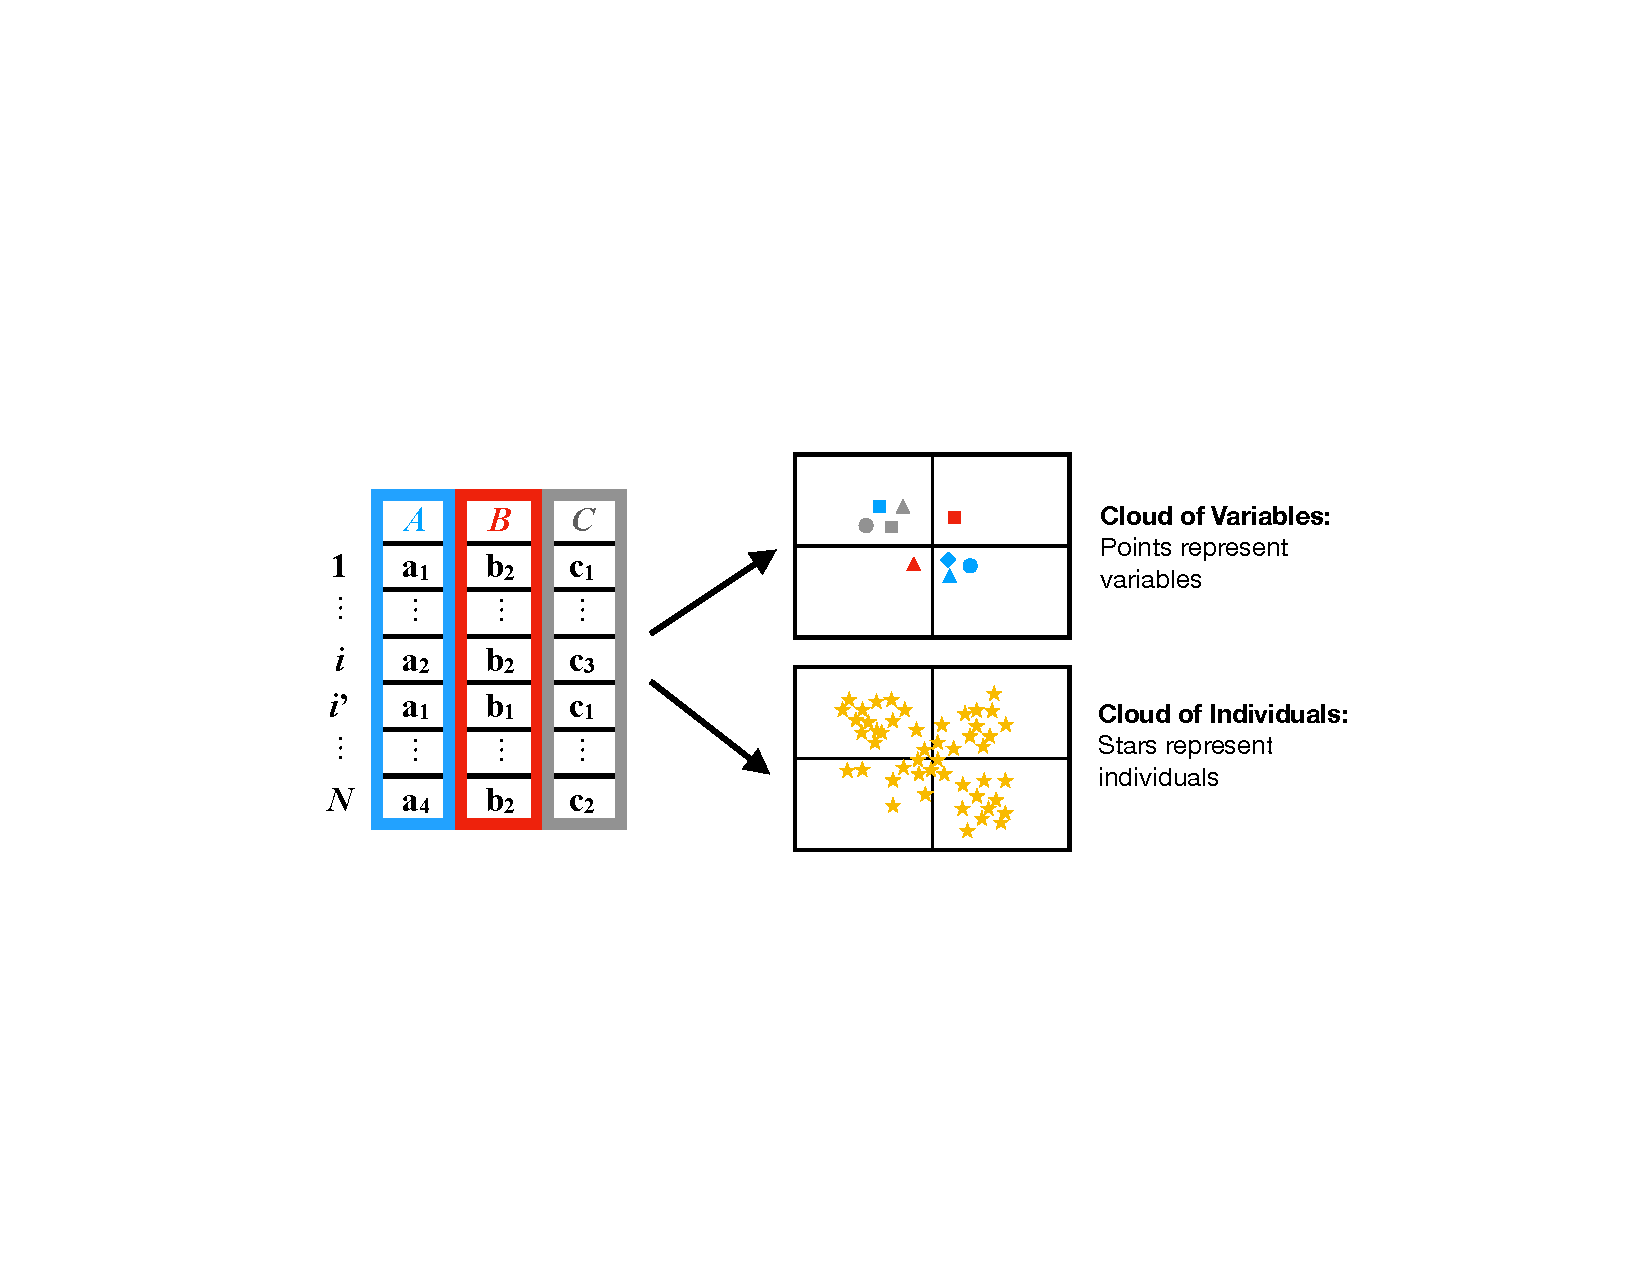
\includegraphics[width=3.5in]{../figs/mcaIdeaNew.pdf}
\caption{Clouds of points generated by MCA}
\label{fig:fig_MCAillustration} 
\end{figure}

Square distance between two correspondents

The squared distance between two respondents is calculated using the
variables for which each had chosen different categories.

\begin{equation}
\begin{aligned}[b]
\label{eq:distInd}
d^2(i, i^{\prime}) &= \frac{1}{Q} \sum_{k\in K} \frac{(\delta_{ik} - \delta_{i^{\prime}k})^2}{f_k}  
\end{aligned}
\end{equation}

where \(\delta_{ik} = 1\) if \(i\) has chosen \(k\) and \(0\) otherwise.
Notice that the smaller the frequencies of disagreement categories, the
greater the distance between individuals. The set of all distances
between individuals determines the cloud of individuals consisting of
\(N\) points in a space with dimensionality \(L\leq K - Q\)
\cite{greenacre2006multiple} (it is assumed here that \(N > L\)).
Additionally, if respondent \(i\) chooses infrequent categories, then
the point \(M^i\) representing individual \(i\) is far from the mean
center of the cloud \(G\). The squared distance from point \(M^i\) to
\(G\) is given by

\begin{equation}
\begin{aligned}[b]
\label{eq:distGM}
(GM^i)^2 &= \left( \frac{1}{Q} \sum_{k\in K} \frac{\delta_{ik}}{f_k}  \right) -1
\end{aligned}
\end{equation}

In the cloud of categories, a weighted cloud of K points, category k is
denoted by point Mk with weight nk: For each question, the sum of the
weights of category points is N, and the relative weight pk of point Mk
is simply pk = fk=Q.

Given two categories k and k0, the squared distance between thee points
MK and Mk0 is calculated as

\begin{equation}
\begin{aligned}[b]
\label{eq:distCat}
(M^k, M^{k^{\prime}})^2 &= \frac{n_k + n_{k^\prime} - 2 n_{kk^\prime} }{n_k n_{k^\prime}/N}
\end{aligned}
\end{equation}

with \(n_{kk^\prime}\) denoting the number of respondents who have
chosen both categories \(k\) and \(k^\prime.\)

The contribution of a category point \(M^k\) to the overall variance is
the ratio of the amount of the variance of the cloud due to category
\(k\). The contribution of a question \(q\) is the sum of the
contributions of its categories. Contributions can be calculated as
shown below:

\begin{equation}
\begin{aligned}[b]
\label{eq:contribMk}
\text{Ctr}_k &= \frac{1-f_k}{K-Q}, \quad \text{Ctr}_q &= \frac{K_q -1 }{K-Q}
\end{aligned}
\end{equation}

THE HEALTH AND RETIREMENT STUDY (HRS) DATASET

Created in 1990 and launched in 1992 by the National Institute on Aging
(NIA) and Social Security Administration, the Health and Retirement
Study (HRS) surveys collect every two years of data from more than
22,000 Americans over 50 years old. It is the first longitudinal study
of Americans approaching the economic and health aspects in the same
survey and being the largest nationally representative multidisciplinary
panel study of Americans aged 50 and older. The study was created and
maintained by the Institute for Social Research (ISR) Survey Research
Center (SRC) at the University of Michigan.

RESULTS AND DISCUSSION

\begin{enumerate}
\def\labelenumi{\arabic{enumi}.}
\tightlist
\item
  Multiple Correspondence Analysis
\end{enumerate}

MCA was performed on a combined dataset from respondents of the 2008 and
2010 waves. Notice that the participants of the 2008 survey are
different than those from the 2010 survey. The clouds patterns for every
wave were examined to confirm that the overall geometric representations
were similar regardless of the number of participants in each wave, or
the year in which the survey responses were collected.

\begin{table}[H]
\caption{Response frequencies (absolute $n_k$ and relative $f_k$), and contributions ($\text{Ctr}_k$) of  top categories by $\text{Ctr}_k$ and levels} 
\centering
\begin{tabular}{lrrr}
  \hline
  Category & nk & fk & ctrk \\ 
  \hline
  sophisticated\_Not at all & 2159 & 0.22 & 0.0093 \\ 
  imaginative\_A lot & 3109 & 0.32 & 0.0081 \\ 
  creative\_A lot & 2668 & 0.27 & 0.0086 \\ 
  caring\_A little & 345 & 0.04 & 0.011 \\ 
  talkactive\_A lot & 2823 & 0.29 & 0.0085 \\ 
  friendly\_A little & 372 & 0.04 & 0.011 \\ 
  careless\_Some & 993 & 0.10 & 0.011 \\ 
  responsible\_Some & 1729 & 0.18 & 0.0098 \\ 
  responsible\_A little & 236 & 0.02 & 0.012 \\ 
  nervous\_Not at all & 3101 & 0.32 & 0.0081 \\ 
  worry\_Not at all & 1625 & 0.17 & 0.0099 \\ 
  moody\_Some & 1470 & 0.15 & 0.01 \\ 
   \hline
\end{tabular}
\label{tab:fknkTop12}
\end{table}

\begin{figure}[h!] 
\centering 
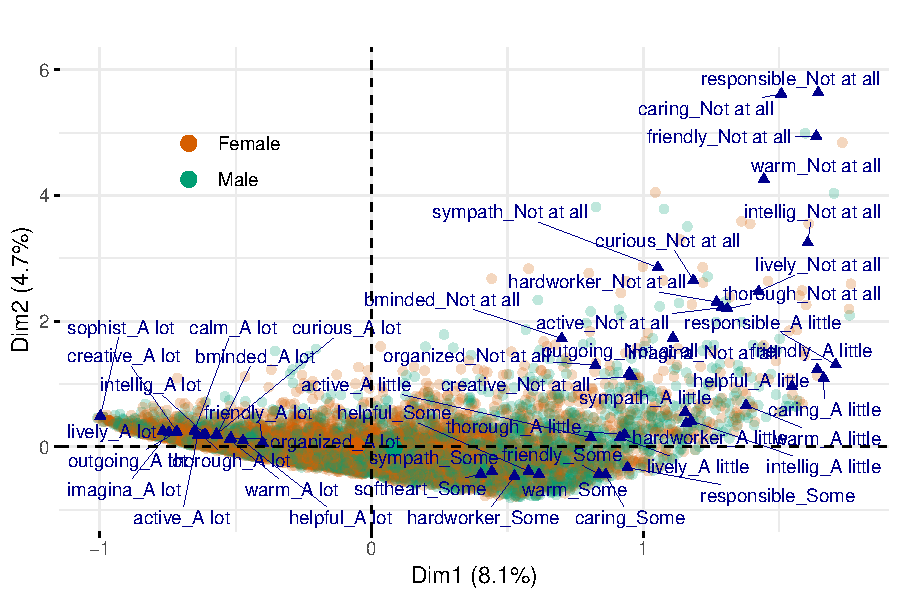
\includegraphics[width=3in]{../figs/newbiplot12.pdf}
\caption{Projection onto the first two principal dimensions}
\label{fig:biplot} 
\end{figure}

Fig. 4 shows the percentages of variance of the first 10 dimensions. The
first principal axis explained 8.11\% of the principal inertia, the
second principal axis explained 4.72\%, and none of the remaining
principal axes explained more than 3\%. Using the modified variance
rates l one can see that the first two dimensions explain about 86.8\%
of the variance in the data.

\begin{figure}[!ht] 
\centering 
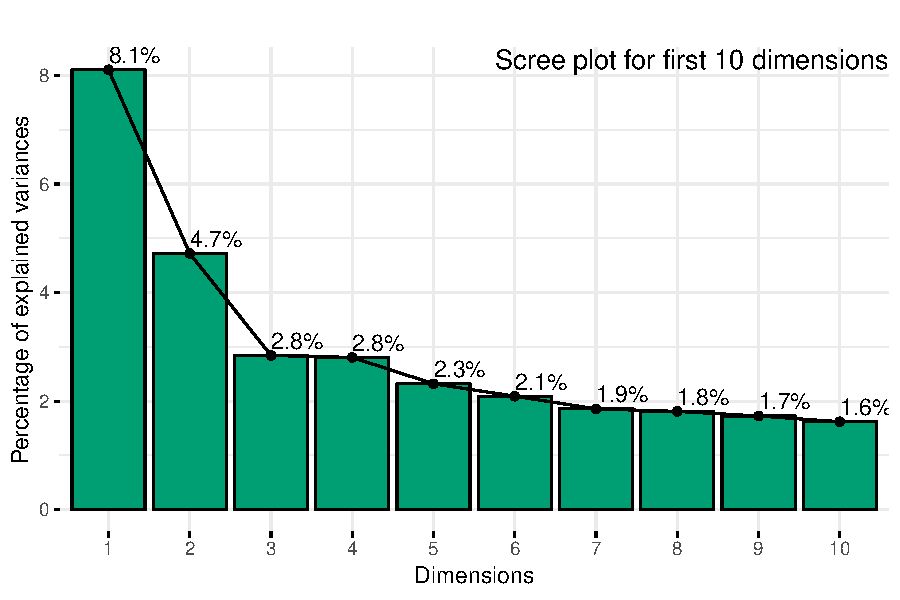
\includegraphics[width=3in]{../figs/screeplot.pdf}
\caption{Variation explained by each principal component}
\label{fig:screeplot} 
\end{figure}

\begin{enumerate}
\def\labelenumi{\arabic{enumi}.}
\tightlist
\item
  Clustering
\end{enumerate}

Geometric data analysis methods have the potential to be used as a
pre-processing step for clustering, given the representation in a lower
dimensional space provided by the principal component technique of
choice. In this work, a hierarchical clustering algorithm is performed
using the coordinates of each respondent in the lower dimensional space
generated by the MCA procedure.

The findings of this hierarchical clustering confirm a natural grouping
for the participants of the survey: the tendency of survey respondent to
use the levels of agreement with the different questions that are part
of the questionnaire, namely, ``a lot'', ``not at all'', ``some'' and
``a little''. These levels of agreements are well separated in distinct
regions within the plane of the first 2 principal dimensions.

\begin{figure}[h!] 
\centering 
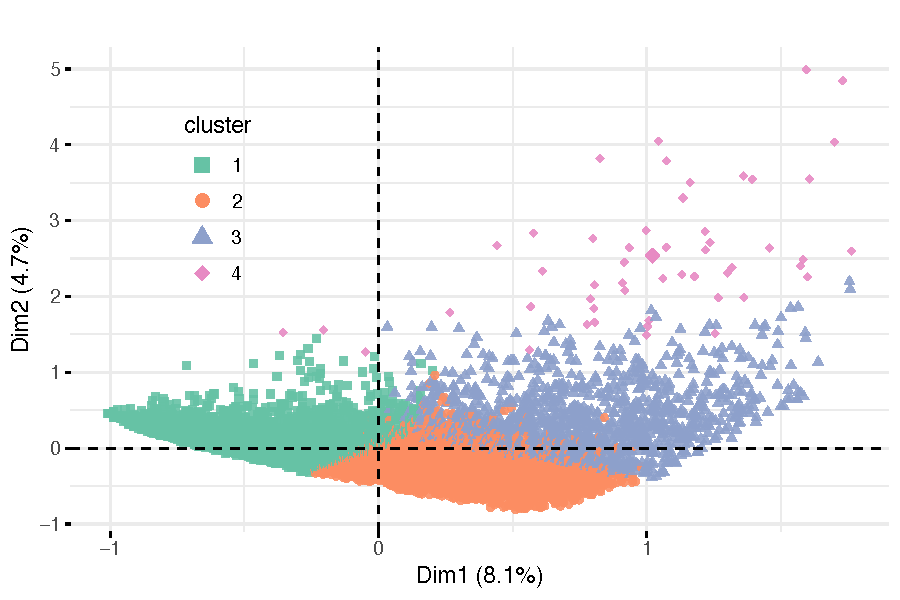
\includegraphics[width=3.2in]{../figs/new_hclust.pdf}
\caption{Hierarchical clustering using principal dimensions generated by multiple correspondence analysis.}
\label{fig:hclust} 
\end{figure}

Hierarchical clustering using principal dimensions generated by multiple
correspondence analysis.

V. Conclusions

The use of unsupervised techniques presented in this work represents an
opportunity to extract valuable insights from longitudinal datasets like
the one made available by the US Health and Retirement Study. MCA allows
for new interpretations and discovery of patterns that take advantage of
the qualitative nature of the data collected from survey respondents.
The hierarchical clustering technique applied to the low dimensional
representation of participants, provided by the MCA method, suggested a
reasonable separation of the respondent profile as

characterized by a personality scale. Results provided by this approach
may be used to explore other areas that have yet to be captured using
the items in the questionnaires, helping in the design of the survey and
sampling procedure, and allowing for correlation studies with other
physical and mental health indicators.

References

Acknowledgements

The HRS (Health and Retirement Study) is sponsored by the National
Institute on Aging (grant number NIA U01AG009740) and is conducted by
the University of Michigan. The HRS has been approved by the
Institutional Review Board at the University of Michigan. The HRS
obtains in- formed verbal consent from voluntary participants and
follows strict procedures to protect study participants from disclosure
(including maintaining a Federal Certificate of Confidentiality). The
public data, made available to registered researchers and used in this
study, is de-identified.


\end{document}
